\subsection{Program Simulation}

The program simulation is based on \jcl semantics, most Java bytecodes can be translated directly to \jcl but type information is lost. Because \jcl has operational semantics defined, it eases the implementation of the simulation, since each instruction is clearly defined.\\\\
When representing Java bytecode in UPPAAL we have chosen to represent an instruction, such as \texttt{aload a} and \texttt{dup}, as UPPAAL locations. 
This implies that a change in the program counter is a change of the location. 
In turn this means that when an instruction is to be executed, the change to the program configuration \textit{Conf} from  \cref{sec:semintro} occurs on the edge to next location.

\begin{minipage}{\linewidth}
\begin{lstlisting}[caption=Java code sample.]
public class Sample{
    public class Sample{
        public static void main(String[] args) {
            install();
            foo(3);
        }
        public static int foo(int i){
            return i != 0 ? 1 : 2;
        }
    }
}
\end{lstlisting}
\end{minipage}
\begin{minipage}{\linewidth}
\begin{lstlisting}[caption=Bytecode sample.]
public static int foo ( int 0 ) ;
   0. iload 0
   1. ifeq 7
   4. iconst 1
   5. goto 4
   8. iconst 2
   9. ireturn
\end{lstlisting}
\end{minipage}

\begin{figure}
\begin{subfigure}{\textwidth}
	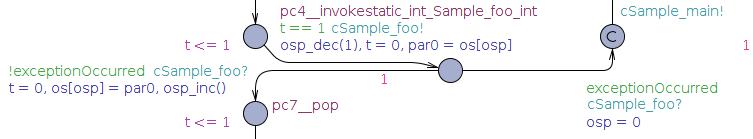
\includegraphics[width=\textwidth]{reportExamples/demo1}
	\caption{Method call in \texttt{main}.}
\end{subfigure}
\begin{subfigure}{\textwidth}
	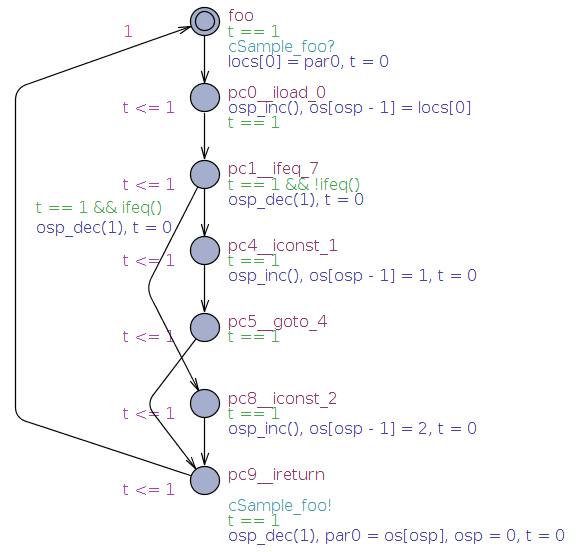
\includegraphics[width=\textwidth]{reportExamples/demo2}
	\caption{the method \texttt{foo}.}

\end{subfigure}

\caption{Auto generated model, Example of \texttt{foo} method.}
\label{fig:fooMethod}
\end{figure}


\subsubsection{Simple Instructions}
\begin{figure}[H]
\centering
\begin{subfigure}{.3\textwidth}
  \begin{lstlisting}
0. iload 0
1. ifeq 7
...
  \end{lstlisting}
  \caption{Java Bytecode Sample.}
\end{subfigure} 
\hspace{10px}
\begin{subfigure}{.6\textwidth}
  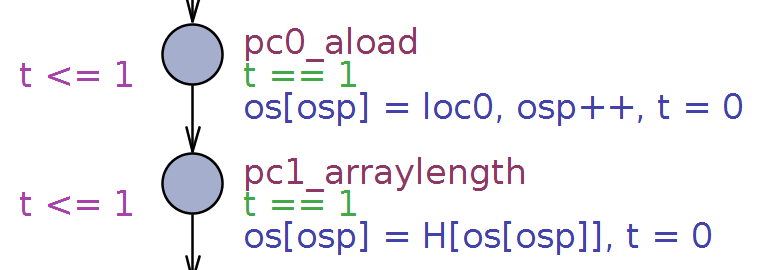
\includegraphics[width=\textwidth]{UPPAAL1.png}
  \caption{Generated model from Sample.}
\end{subfigure}
\caption{Java bytecode and corresponding UPPAAL model.}
\label{fig:uppaal1}
\end{figure}

\Cref{fig:uppaal1} shows how two Java Bytecode instructions are represented in UPPAAL. On the left we see the Java bytecode, the first line with program counter 0 we have the \texttt{iload 0} instruction. \texttt{iload 0} pushes a integer to the top of the operation stack from local variables at position zero, then increments the operand stack pointer and program counter.\\\\
%uppaal location edge
In UPPAAL the location \UPP{pc0\_iload\_0} represents \texttt{iload 0}. The UPPAAL model is seen in \Cref{fig:uppaal1}b. We simulate execution time with the location invariant \UPP{t <= 1} and guard \UPP{t == 1} on the edge leading to the next location. The guard is found right below the location name right of the edge and invariant is to the left of the edge. In this sample we defined the execution time as 1 time unit.\\\\
In the update on the edge seen below the guard, we simulate the data flow by assigning the value of the local variable \UPP{loc0} to the top of the operand stack \UPP{os} represented by operand stack pointer \UPP{osp}. \UPP{osp} is incremented as the operand stack grows, the increment of the program counter is simulated by the edge itself.

\subsubsection{Jumps and Branches}
For the majority of instructions the program counter is set to the next instruction after execution, but for a jump with \texttt{goto a} the edge goes to the instruction with the program counter corresponding with value of \texttt{a} as seen in \Cref{fig:fooMethod}.

Conditionals such as \texttt{if\_cmpeq a} are modelled by a location having two outgoing edges, see \Cref{uppaal1}, one to the next instruction and one for the program counter of with and offset of \texttt{a}. On these edges the guard is used to determine which of the edges is to be traversed.

\subsubsection{The Operand Stack, Local Variables and the Heap}
To simulate the operand stack, we use an operand stack pointer to point at the next free position in an array. Local variables and the heap are both represented as arrays in the UPPAAL model, but they do not use an explicit pointer to access them since access to these are not necessarily performed in a top-down manner as with the operand stack.

\subsection{Method Calls}\label{subsubsec:method}
Method calls covers the Java bytecode instructions: \texttt{invokestatic} for static calls, \texttt{invokespecial} for class constructors and private calls, and \texttt{invokevirtual} virtual calls. To illustrate how these instructions are modelled, we use the Java code sample in \cref{lst:virtual}.
\begin{lstlisting}[caption={\texttt{Bclass} extends \texttt{Aclass}, \texttt{Aclass} implements the methods foo and bar, and \texttt{Bclass} overwrites foo.}, label={lst:virtual}]
public class Virtual{
  public Aclass a;
  public Aclass b;

  public Virtual(){
    a = new Aclass();
    b = new Bclass();
    int ia = a.foo() + a.bar();
    int ib = b.foo() + b.bar();
  }
}
\end{lstlisting}
The sample includes the bytecode instructions \texttt{invokespecial} and \texttt{invokevirtual}.
\texttt{invokestatic} is omitted as \texttt{invokestatic} and \texttt{invokespecial} are nearly identical, with the only difference being if an object reference from the operand stack is parsed as a parameter.
As such all methods call can be divided into two categories, virtual and static.\\\\
These categories are defined in the Java specification: ``Virtual methods are instance methods that are resolved dynamically. The set includes all public, protected and package-visible instance methods. Private instance methods and all constructors are not virtual methods, but instead are resolved statically during compilation.''~\cite[chap. 4.3.7.6]{java_card_spec}

\subsubsection{Static Methods}
Static method calls, as shown in \cref{fig:invokespecial}a, are represented by three additions to the model. These additions consist of locations and edges.\\\\ 
%, but they do not have any associated program counter since they are not a part of the original program.\\ what?
% caller
The first is a new location in the caller for every method call it performs. This makes it possible to simulate parameter passing from the caller, as well as control transfer when waiting for a callee to return control after a method call. The simulation of the caller remains in this location until the callee returns control, after its simulation has finished. This control transfer is modelled with a synchronisation on the edge, going from the new state in the caller and back to its original control flow, as seen in \cref{fig:invokespecial}b.\\\\
% callee
The second is an addition of one additional location in every template. The first, initial location, \texttt{Aclass}, in \cref{fig:invokespecial}c, serves two purposes: it enables the control transfer from the caller to itself by synchronisation, and simulates passing of arguments into the method from the caller.\\\\
% main case and return
The third is the edge from the \texttt{return} instruction, seen in \cref{fig:invokespecial}c. This is one of the two edges pointing to the \texttt{AClass} initial location, and the other is for exceptions, which are covered in \Cref{sec:exceptions}. For main, the edge goes to a \textit{Done} location instead of the initial location, where the simulation ends when it has finished. For other templates, this is where control is transferred back to the caller, and the edge goes to the initial location.


\begin{figure}[H]
\centering
\begin{subfigure}{\textwidth}
  \begin{lstlisting}
...
9. invokespecial void Aclass.<init> ( )
12. putfield Virtual.a : Aclass
...
  \end{lstlisting}
  \caption{Invokespecial Bytecode generated by Sawja.}
\end{subfigure} \\
%\hspace{10px}
\begin{subfigure}{.65\textwidth}
  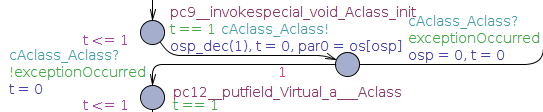
\includegraphics[width=\textwidth]{invokespecial.png}
  \caption{Invokespecial Instruction.}
\end{subfigure}
\hspace{10px}
\begin{subfigure}{.25\textwidth}
  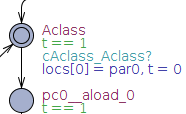
\includegraphics[width=\textwidth]{initloc.png}
  \caption{Initial Location.}
\end{subfigure}
\caption{Java bytecode and corresponding UPPAAL model.}
\label{fig:invokespecial}
\end{figure}


\subsubsection{Virtual Methods}
Virtual methods are similar to static methods in regards to representation in the method template for caller and callee, but instead of handling control directly to callee method templates, a template responsible for resolving the virtual call is inserted for this purpose.
\cref{fig:invokevirtual} is the resolver template generated for the code in \cref{lst:virtual}, there is a total of three virtual methods in this sample and the resolver has a waiting location for each.\\\\
Every class is mapped to an integer $clID$ and an array, $classHierarchy$, represents the class hierarchy of the program. The initial location \UPP{Invoke} waits for a synchronisation, after which the location \UPP{Resolver} has an outgoing edge for every possibility, in this sample that is five. There are essentially always three distinct possibilities 

\begin{itemize}
\item There are no methods and no super where $clID == 0$.
\item There is a method matching the class and method signature. In this case, call the method.
\item There are no methods but there is a super class, then assign $clID = classHierarchy[clID]$ and try again.
\end{itemize}

This is based on $methodLookup$ from the \texttt{INVOKEVIRTUAL} semantics from \cref{app:invokevirtual}.

 
\begin{figure}[H]
\centering
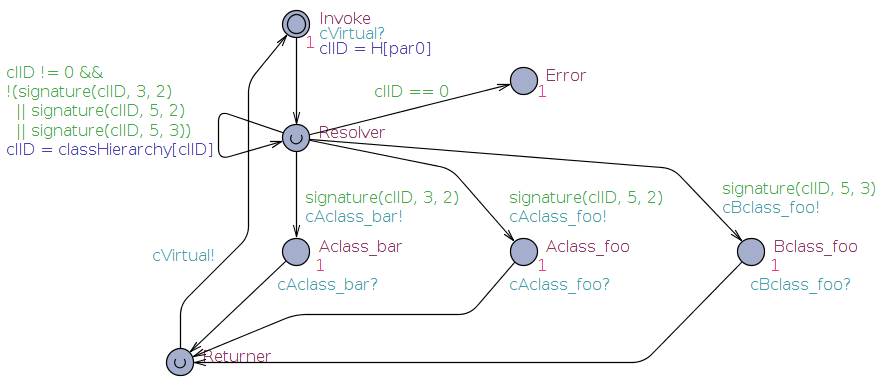
\includegraphics[width=\textwidth]{invokevirtual.png}
\caption{Invokevirtual.}
\label{fig:invokevirtual}
\end{figure}

\subsubsection{Exceptions}
\label{sec:exceptions}
\kri{is this the right place?, and reread, and figures}
Exceptions are handled by try catch blocks which does not have a corresponding bytecode instruction, instead they defined at the end of a method as seen in \cref{lst:exception}, \texttt{0, 8, 11} represents the corresponding program counters (pc). When exceptions are thrown by the \texttt{athrow} instruction, there are two outcomes, either there is some exception handling covering the \texttt{athrow} defined in the current method, in which case the execution continues from the \texttt{catch start} pc. If there is no exception handling covering the \texttt{athrow}, the top stack frame will be poped and the process repeat, no handling and the new top frame is poped. On \jc an unhandled exception by the applet can be used to indicate an error such as \textit{noaccess}.



\begin{figure}
  \begin{lstlisting}
....
try start: 0; try end: 8: catch start: 11; catched type: java.lang.Exception.
  \end{lstlisting}
  \caption{Invokespecial Bytecode generated by Sawja.}
  \label{lst:exception}
\end{figure}



